\subsection{Introduction}
Graph Theory is one of the main instrument used for inferring how brain works.
A graph is a mathematical object defined combining \textbf{nodes} \(V\) (or vertices) and \textbf{edges} \(E\) (or arcs), that connect nodes.
\begin{figure}[H]
    \centering
    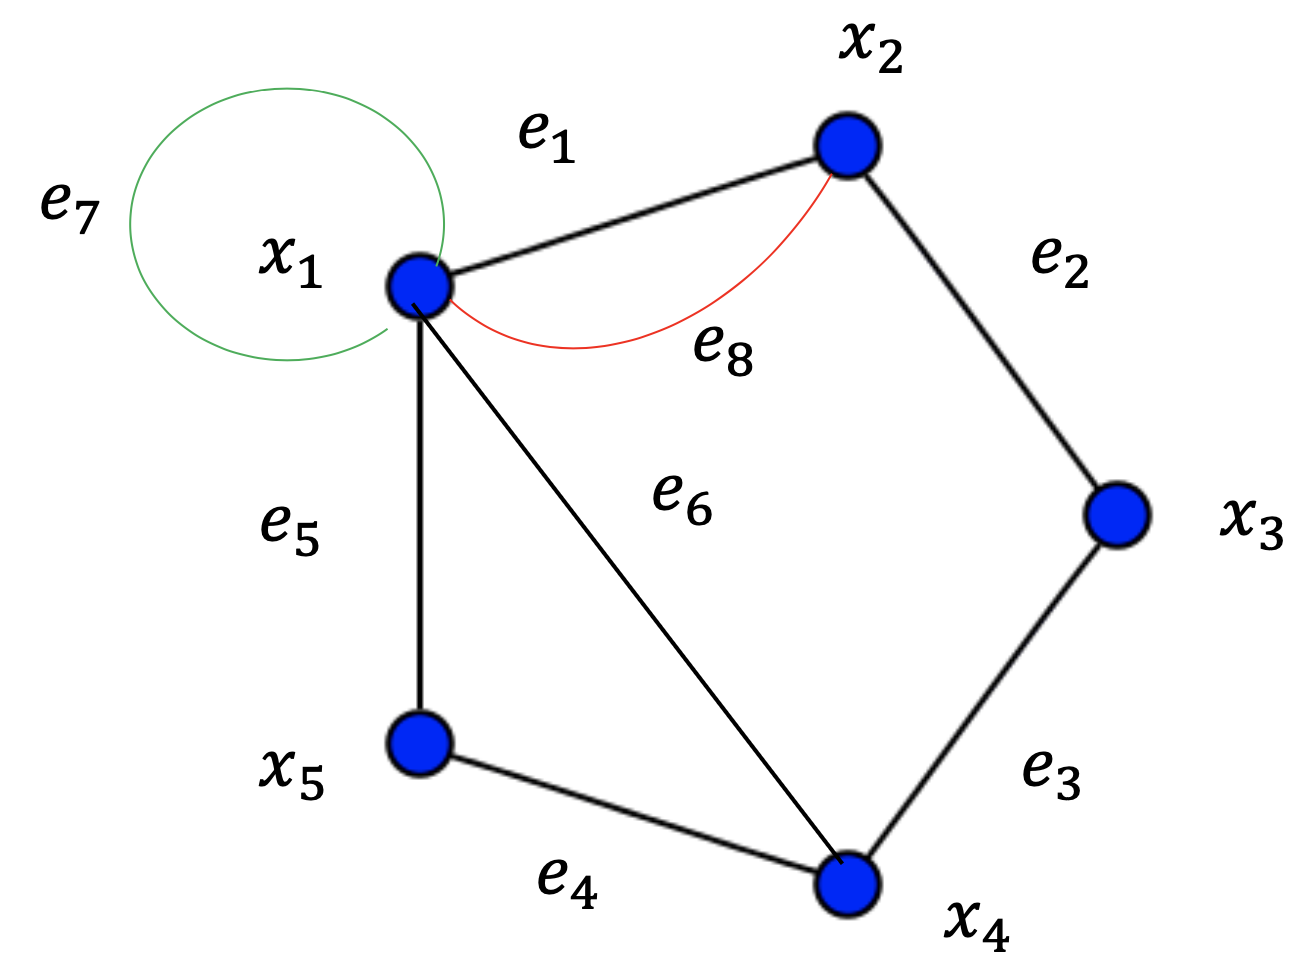
\includegraphics[scale=0.25]{15_1.PNG}
\end{figure}
\begin{equation*}
    G=(V,E)
\end{equation*}
\begin{equation*}
    V=\{x_1, x_2, ..., x_n\}
\end{equation*}
\begin{equation*}
    E=\{\{x_1, x_2\}, \{x_2,x_3\},..., \{x_\{n-1\},x_n\}\}
\end{equation*}
\subsubsection{Definitions}
\begin{enumerate}
    \item A node \(x_i\) is adjacent to \(x_j\) if they are connected by an edge.
    \item An edge \(e\{x_i, x_j\}\) is incident to \(x_i\) and \(x_j\) being a connection between the two nodes.
    \item The number of edges incident to a node is called the \textbf{degree} of the node.
    \item A graph \(G=(V,E)\) with no loop or multi-edges is called \textbf{simple} (all our graph will be simple).
    \item An edge \(e\{x_i,x_i\}\) incident to the same node \(x_i\) is called a \textbf{loop}.
    \item Two or more edges \(e\{x_i,x_j\}\) incident to the same pair of nodes are called \textbf{multi-edges}.
\end{enumerate}
\subsection{Common Graphs}
There are many different topographies depending on the number of nodes and on how they are connected. 
\begin{figure}[H]
    \centering
    \subfigure[]{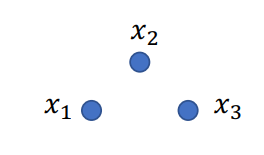
\includegraphics[width=0.2\textwidth]{15_2.PNG}} 
    \subfigure[]{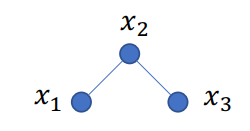
\includegraphics[width=0.2\textwidth]{15_3.PNG}}
    \subfigure[]{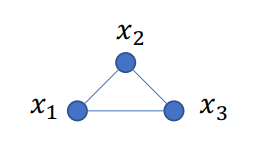
\includegraphics[width=0.2\textwidth]{15_4.PNG}} 
    \subfigure[]{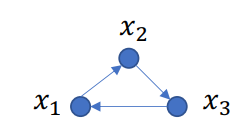
\includegraphics[width=0.2\textwidth]{15_5.PNG}}
\end{figure}
\begin{itemize}
    \item \textbf{Null or empty graph}: formed only by nodes and no edges.
    \begin{equation*}
        E=\emptyset
    \end{equation*}
    \item \textbf{Binary Graph}: each edge has two possible values: 0 or 1. 0 means that it is not present and 1 that it is present.
    \begin{equation*}
        E=\{\{x_1, x_2\}, \{x_2,x_3\},..., \{x_\{n-1\},x_n\}\},\hspace{0.5cm}e\in[0,1];
    \end{equation*}
    \item \textbf{Weighted Graph}: every edge is connected to the others (graph fully connected).
    \begin{equation*}
        E=\{\{x_1, x_2\}, \{x_2,x_3\},..., \{x_\{n-1\},x_n\}\},\hspace{0.5cm}e\in[0,\infty];
    \end{equation*}
    \item \textbf{Directed Graph}: every edge is connected to the others (graph fully connected), and info on the direction of the connection is present.
    \begin{equation*}
        E=\{\{x_1, x_2\}, \{x_2,x_3\},..., \{x_\{n-1\},x_n\}\},\hspace{0.5cm}e\in[-\infty,\infty];
    \end{equation*}
\end{itemize}
PLV and Coherence are weighted graph, because are symmetric and don't contain info about directionality.
\subsection{Connectivity Matrices and Brain Graphs}
How do we compare brain observations between different scales? Graphs are a tool to collect an abstract representation, that allows to compare network properties independently of the scale at which they have been observed (at the single neuron level or at the network level, for instance) and to compare between signals obtained using different modalities (i.e., fMRI, electrophysiology and metabolic imaging).\\
A very important point is hence how to construct a brain graph. The simplest definition would be to have nodes coincident with the neuronal ensembles that are being recorded. However, the situation becomes more complicated when multiple recordings are combined. Nodes can in fact be micro-, meso- and macro-scopic, and it's always possible to make comparisons across scales but it's first necessary to understand how nodes are defined in each one and how this definition is related to the one in the other scales.\\
The simplest way to represent nodes is using \textbf{adjacency matrices}, that are matrices that define the pair-wise correlation between every node in the network.
\begin{figure}[H]
    \centering
    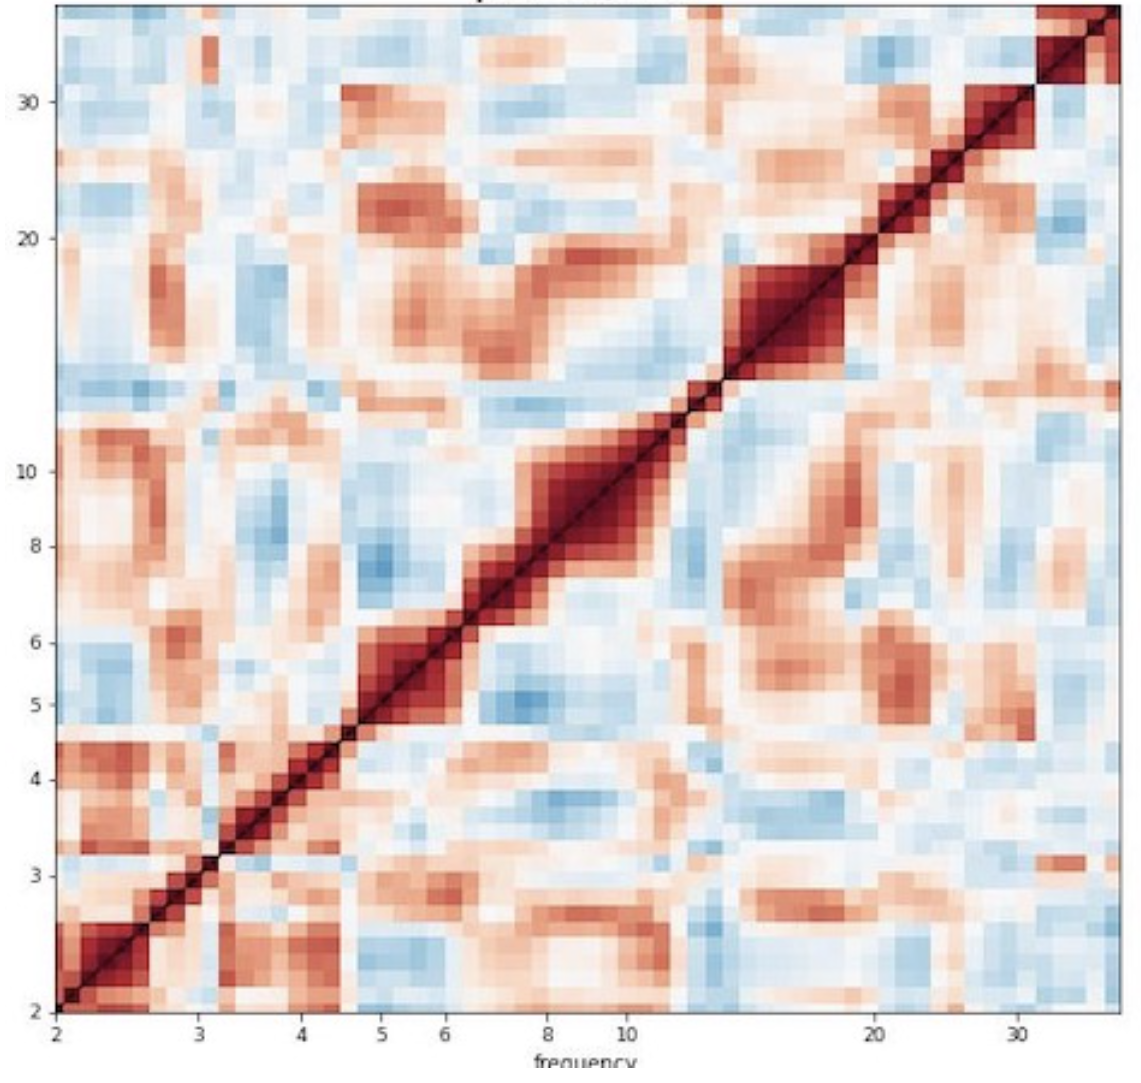
\includegraphics[scale=0.15]{15_6.PNG}
\end{figure}
A typical adjacency matrix of a brain network shows the highest values of correlation near the diagonal, where the close electrodes show the largest correlation, and then there are clusters of connections that show the correlation between long-range brain areas.\\
If the matrix doesn't show this hierarchical modular structure, there is an error in the algorithm or there is some pathological condition.\\
Starting from this matrix, a lot of information can be extracted.
\subsubsection{Measures of node connectivity}
The node connectivity represents how a single network in the graph is connected to all the others. The simplest way to evaluate it is to compute the node degree.\\
The \textbf{node strength} or degree is the sum of the edge weights of the edges connected to a specific node:
\begin{equation*}
    s_i=\sum_{i\neq j}w_{i,j}
\end{equation*}
The \textbf{network density} is the number of edges that are present (different from 0) in all sets of possible edges. It only make sense in binary graphs, because in weighted graphs all nodes are connected to all the others and there is just a difference in the weight
\begin{equation*}
    |E|=\sum_{i=1}^{N} k_i
\end{equation*}
\textbf{Clustering coefficient} of a single node \(i\) is the number of nodes \(j\) that are both adjacent to \(i\) and adjacent to each other. It tells us how much one node is central for our network, so how modular is the network.
\subsubsection{Degree Distribution}
It's the probability of having one node connected to other nodes.
It applies very well to large (\(>1000\)) networks. 
By looking at it, info about the actual topography of a network can be inferred.
In \textbf{single scale graphs} (Erdos-Renyi) the degree distribution follows a binomial distribution that for large n tends to a gaussian. 
\begin{align*}
    Pr(deg(x)=k) &= \begin{pmatrix}
    N+1 \\
    k
    \end{pmatrix}
    p^k(1-p)^{N-1-k}
\end{align*}
For \textbf{scale free graphs} (brain and all biology inspired systems) follow a power law distribution, suggesting the presence of large hubs (nodes very connected, like Fiumicino airport).
\begin{equation*}
    Pr(deg(x)=k)=k^{-\alpha}
\end{equation*}
For \textbf{broad-scale graphs} (social network) follow a truncated power law (combination of exponential and binomial).
\begin{equation*}
    Pr(deg(x)=k)=k^{-\alpha}e^{-k/k_c}
\end{equation*}
\subsubsection{Centrality and Hubs}
Looking at scale-free distributions, it can be deduced that some nodes have a very important role in sustaining the stability of the network. Hubs have a very high clustering coefficient, because they are connected to all the nodes: the majority of the nodes can communicate with each other only passing through the hubs.\\
So, central nodes have 3 properties:
\begin{enumerate}
    \item maximum possible degree
    \item are included in the shortest possible topological path between two other nodes
    \item are located at the shortest distance from all other nodes.
\end{enumerate}
In brain networks an example can be made considering surgery in epileptic networks, in which nodes that are central for propagation or creation of epilepsy are looked for and removed or disconnected from the network.\\
Based on these observation, the three cardinal aspects of \textbf{centrality} are: degree, betweenness and closeness. 
These are used to easily identify these regions.
\begin{itemize}
    \item \textbf{Degree centrality} is equivalent to node degree.
    \item \textbf{Eigen-vector centrality} takes into account the degree of a node and those of its neighbors is computed by eigen-decomposing it:
    \begin{equation*}
        C_e(i)=\frac{1}{\lambda_1}\sum_{j=1}^NA_{ij}x_j
    \end{equation*}
    \item \textbf{Closeness Centrality} is the inverse of the average shortest path length, that is the shortest number of edges that one has to perform to go from one to another side of the network. 
    \begin{equation*}
        C_c(i)=\frac{N-1}{\sum_{j\neq i}l_{ij}}
    \end{equation*}
    \item \textbf{Betweenness Centrality} measures the proportion of shortest paths between all node pairs in a network passing through a given node. So it measure how much a single node is in between to large population. 
    \begin{equation*}
        C_b(i)=\frac{1}{(N-1)(N-2)}\sum_{h\neq i,h\neq j, j\neq i} \frac{\rho_{hj}(i)}{\rho_{hj}}
    \end{equation*}
\end{itemize}
So, as already said, biological networks are characterized by skewed degree distributions that point to the existence of highly connected nodes called hubs. How can they be detected in brain networks?\\
Sporns (2007) suggested that they should have: 
\begin{enumerate}
    \item high degree, so are connected to many nodes;
    \item high closeness centrality, so support communication between nodes;
    \item high betweenness and low clustering, so support integration of unconnected nodes.
\end{enumerate}
Van den Heuvel (2010) used a similar approach to classify brain regions based on their centrality with respect to the human connectome for each node. The node is central if:
\begin{enumerate}
    \item The node is ranked in the top 20\(\%\) among those with highest degree.
    \item The node is ranked in the top 20\(\%\) among those with highest betweenness.
    \item It is in the bottom 20\(\%\) with the lowest clustering coefficient.
    \item It is in the bottom 20\(\%\) among those with the lowest average path length.
\end{enumerate}
\subsection{Graphs Interpretation and Labeling}
Interpreting graphs is usually very difficult, because often a lot of nodes are connected together. So, to extrapolate some info from them, it's necessary to perform some labeling in a meaningful way.\\
To do it, labels are assigned basing on the property of the nodes. In brain networks modules are looked for, that are clusters of nodes sharing some properties.
\subsubsection{Modularity}

\begin{figure}[H]
    \centering
    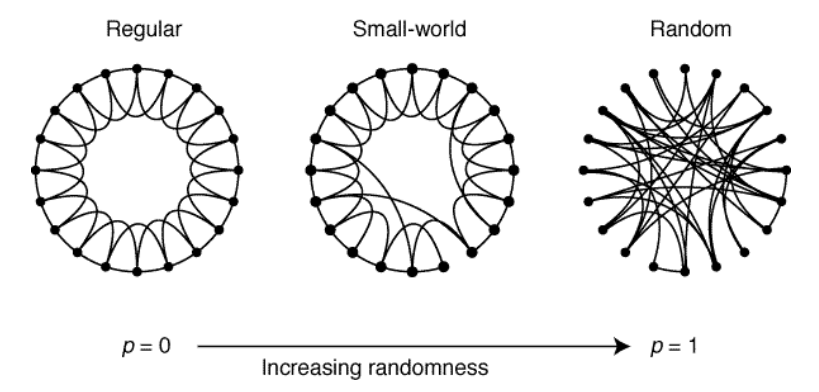
\includegraphics[scale=0.7]{15_7.PNG}
\end{figure}

Modular networks (and also the human brain) generally have small-world properties, such as high-clustering coefficients and low characteristic path lengths. \\
This means that there is a group of nodes that are highly connected and then an hub, so that the information can reach all possible other portion of the network passing through this hub. This is optimal for energy conservation, speed of communication and general economy of the brain.\\
The basic idea to perform modularity is to reduce a large set of observations across different measures into a smaller subset of informative clusters. However, the number of natural clusters is not known a priori. Hence, techniques like multidimensional scaling or PCA are often used. In general, data clustering methods can be divided in two classes: \textbf{agglomerative} starts from the part in which nodes share the same properties or \textbf{divisive} that starts from a larger view of the network.
\subsubsection{Agglomerative Modularity}
In agglomerative modularity the nodes that share the same properties are combined starting from a small portion of the network.\\
\textbf{Hierarchical clustering} groups nodes in clusters to promote high within cluster similarity and low between cluster similarity. It's an iterative algorithm in which at the beginning all nodes belong to their own cluster, then nodes with the highest similarity and pair of clusters with highest similarity are joined.\\
Two possible implementations are the Average-linkage clustering and Single-linkage or Complete-linkage clustering.
\subsubsection{Divisive Modularity}
In divisive modularity the network is cut in small portions. \\
It's based on betweenness centrality: the betweenness is calculated for each edge in the graph, then the edges that have the highest score are removed (cut the network at that point). Then the process is repeated until there are no more edges in the graph.\\
Depending on where the graph is cut, 2 or 100 clusters can be obtained. When deciding where to cut, some factors can be considered:
\begin{itemize}
    \item Optimize neighboring proximity of nodes.
    \item Use algorithms that provide the confidence intervals (obtained through statistical analyses) on where the network can be cut.
\end{itemize}
So, the usage of agglomerative or divisive modularity is o good way of proceeding, since it does not require an apriori selection of the exact number of clusters that will be extracted from data. However, there is no easy way to determine the quality of the obtained clusters. To do it, often permutations are used to estimate the confidence intervals.
\subsubsection{How can we quantify modularity?}
A high quality partition should have:
\begin{itemize}
    \item Highly-cohesive modules or strongly connected nodes within the same module.
    \item A greater intra-modules connectivity than expected by chance (when edges are placed at random).\\
    To evaluate it, the \textbf{modularity index} can be quantified:
    \begin{equation*}
        Q=\frac{1}{2}A_{ij}\delta(m_i,m_j)
    \end{equation*}
    This value is dependent on the point where the system is cut, so it should be calculated for different thresholds. Then, the value that maximizes the modularity is chosen.\\
    The Louvain method is an algorithm that can be used to maximize the modularity index.
\end{itemize}

\subsection{Null Models}
As already introduced for PLV or PSTH, the evaluation of a single parameter is meaningful only in presence of a null hypotheses. This means that measuring a clustering coefficient of the brain network of 0.4 and an average path length of 4 is not particularly informative in the absence of comparative information (null hypothesis).
In brain networks, in fact, the edges are not placed randomly but in specific anatomical directions. So, a good way to proceed would be to compare the results of our brain network with another random brain network.\\
The simplest form of random network is the Erdos-Renyi model, but also other ones can be used.
\subsubsection{Erdos-Renyi model}
This model is very simple, but it is not very comparable with brain network because it not a small-world network. It has long range connections which are very expensive in terms of energy consumption and topographical characteristics that are very different from the ones that exist in the brain.\\
To build this model:
\begin{enumerate}
    \item Distribute \(N\) nodes in a random topology.
    \item Pick a random (uniform) number between 0 and 1.
    \item If this is greater than \(p\) then draw a wire between \(x_1\) and \(x_2\).
    \item Repeat for all possible \(N\) nodes.
\end{enumerate}
This model actually generates \(2^m\) possible models.
\subsubsection{Watts-Strongatz model}
Here the degree distribution is Poisson like which is unrealistic when compared to real-world network.
\begin{enumerate}
    \item Begin with \(N\) nodes in 2D space positioned on a ring and a desired mean node degree \(\rangle k\langle\). Choose \(\rangle k\langle\) as an even number
    \item Add \(N\rangle k\langle/2\) edges to a given node \(\rangle k\langle/2\) on each side between its \(\rangle k\langle\) nearest neighbors
    \item Randomly rewire each connection with probability \(0<p<1\) avoiding loops and multi-edges.
    \item \(P=0\) yields a Erdos-Renyi model for \(N\) nodes
\end{enumerate}
\subsubsection{Barabasi-Albert model}
This approach yields a graph with a degree distribution that follows a power-law distribution and has a connection density of \(2v/(N-1)\).
\begin{enumerate}
    \item Nodes are not fixed but rather added at each iterations
    \item Begin with a few interconnected nodes.
    \item At each iteration, add a new node with preferential attachment, i.e., a new node added to the graph will preferentially be connected to highly connected nodes already present in the graph. ("rich gets richer")
\end{enumerate}
\subsubsection{Maslov-Sneppen Rewiring}
This model has been defined as a surrogate for comparison with neuronal networks. It was specifically built for binary graphs:
\begin{enumerate}
    \item It takes the graph and iteratively rewires each edge.
    \item At each iteration it randomly selects two edges \(e{x_1,x_2}\) and \(e{x_3,x_4}\)
    \item It then move these links to form \(e{x_1,x_4}\) and \(e{x_2,x_3}\).
    \item If one of the edges already exists, it is dropped.
    \item The algorithm iterates for a fixed number of iterations. This number is suggested to exceed 100 times the number of existing edges.
\end{enumerate}
This method yields a graph with the same size, average node degree and degree distribution as the original one.\\
Its advantage is that it is simple to implement but quite expensive for very large networks.
\subsection{Critical Brain Hypothesis}
The theory of \textbf{self-organized criticality} is part of the statistical mechanics that studies the average behavior of mechanical system where the state of the system is uncertain. Statistical mechanics is a branch of theoretical physics that studies the average behavior of mechanical system where the state of the system is uncertain. Thanks to it, complex system with many (\(10^{23}\))) degrees of freedom can be described.\\
The brain is thought to operate in a \textbf{sub-critical regime near the critical point} in physiological conditions. This critical point is seen as the point of transition between two states.\\
Self-organized criticality (SOC) is a property of dynamical systems which have a critical point as an attractor. In this field, systems are predicted to exhibit scale-invariant characteristics or power-laws.\\
Complex systems can create very complex dynamics. The global behavior of the network originates from local interactions, in absence of a single generator. The dynamic behavior of brain network can be observed with every brain time series. One simple way to do it, is through he large-scale neuronal avalanches.
\subsubsection{Large-scale neuronal avalanches}
In dynamical systems the activity is propagated from one region to another with different travelling waves. Large-scale neuronal avalanches are the simplest way to characterize travelling waves. Neuronal avalanches are described in terms of their spatial extent and life-time. Both these properties follow a power-law in physiological conditions, and when the brain is operating near the critical point. From avalanches the propagation matrix can be extracted.
\begin{figure}[H]
    \centering
    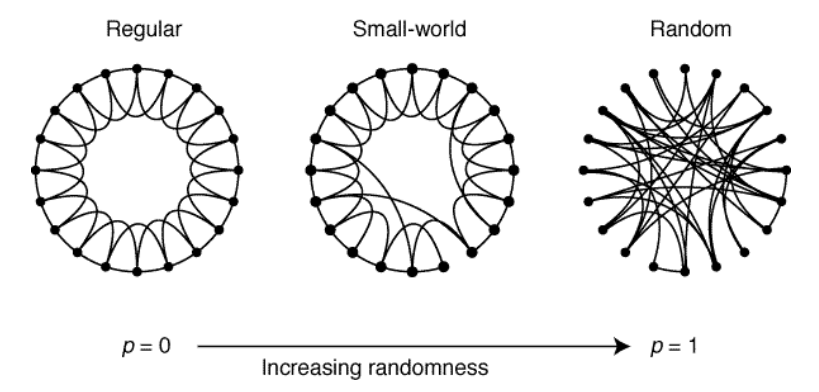
\includegraphics[scale=0.45]{15_8.PNG}
\end{figure}
One way to measure neuronal avalanches in large scale activity can be to look at the activity at different sides of the brain: after filtering in a specific band and taking the module of the complex wavelet, the amplitude dynamics can be extracted. Than an amplitude threshold is defined and only the nodes whose amplitude is above the threshold are considered as active.\\
This is performed for a single value to have a single element of the matrix, or for many time windows and amplitude thresholds in order to quantify the network large activation. In the image, the value in yellow follows exactly a power-law and defines the critical regime (i.e., the portion of the network where the communication is optimal).
\subsubsection{Long-range temporal correlations}
Brain spontaneously generates neuronal oscillations with great variability in terms of frequency, duration and amplitude. Little is known of their long-term temporal structure. But since the brain has memory, the brain should have some sort of long-term temporal correlation.\\
To analyze this quantity, the simplest analysis that can be done is the \textbf{Detrend Fluctuation analysis (DFA)}.\\
This algorithm starts from the assumption that a critical system that works at the optimal state point has the maximum (best) possible DFA. Increasing or decreasing of this value after any particular condition (like cut part of the brain, or sleeping, or moving,...) means that critical point is moving away, going towards more excitatory or inhibitory states.
\begin{figure}[H]
    \centering
    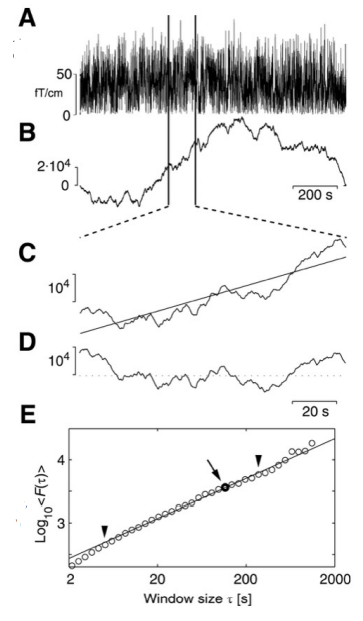
\includegraphics[scale=0.9]{15_9.PNG}
\end{figure}
To realize this algorithm, after measuring the activity in one point, the amplitude modulation is taken (A) and a cumulative distribution of this amplitude generated (B). Then, considering a smaller time window (C), the linear trend within it is quantified and removed (D). It is repeated for different time windows, for which different linear fitting will be obtained. The DFA (E) is defined as the linear or power-law fitting of the curve built from the amplitude dynamics observed at different time windows. This technique is long-range because we look at very large time window (2000 s).\\
When the DFA changes, different interpretations can be hypothesized.
\begin{figure}[H]
    \centering
    \subfigure[]{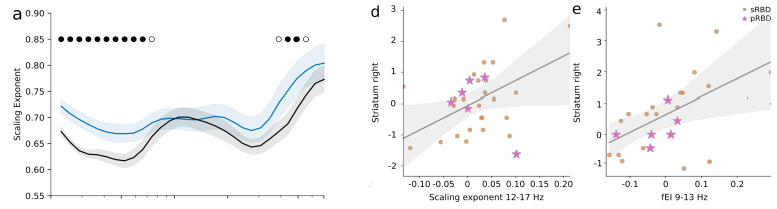
\includegraphics{15_10.PNG}} 
    \subfigure[]{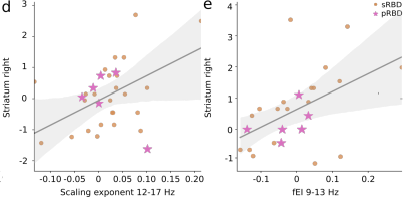
\includegraphics{15_11.PNG}}
\end{figure}
For instance, in this study, the DFA computed across multiple frequencies (2-70 Hz) of patients with a sleeping disorder and healthy controls is observed.\\
These subjects have significantly different values in the low frequency range. This change is correlated with a clinical index in the patients pathology that is the dopaminergic loss: increases of DFA for healthy controls is directly correlated with this loss.


